% !TeX root = ../libro.tex
% !TeX encoding = utf8
%
%*******************************************************
% Introducción
%*******************************************************

% \manualmark
% \markboth{\textsc{Introducción}}{\textsc{Introducción}} 

\chapter*{Conclusiones y vías futuras}
\addcontentsline{toc}{chapter}{Conclusiones} % Añade el glosario a la tabla de contenidos

\section*{Conclusiones}
Con este trabajo se ha intentado transmitir la importancia del teorema sobre variedades topológicas $2$-dimensionales, comprendiendo la dificultad que conlleva su demostración y la gran cantidad de elementos utilizados de la teoría de Morse.\\
\\Se ha desgranado la demostración aportada por Allen Hatcher en su artículo ``The Kirby Torus Trick for Surfaces'', de manera que esté al nivel de un estudiante, pero siempre que se supongan ciertos los resultados utilizados de la teoría de Morse. En caso de querer completarlo podría requerir todo un trabajo exclusivamente para ello.\\
\\La demostración de los resultados del artículo de Allen Hatcher no es complicada ni extensa si nos basamos en los ``Hechos'' que él aporta. Estos hechos son los que verdaderamente requieren un amplio conocimiento de la teoría de Morse. La herramienta trasladada por Allen Hatcher, la técnica del toro de Kirby, junto con tales Hechos han sido la clave para la demostración del ``Teorema de Alisamiento de Asas''.\\
\\He podido apreciar toda una teoría completamente nueva, que daría para una asignatura, y es por esto que he intentado ilustrarla con el programa que he diseñado e implementado.\\
\\Además, dicho programa ha aportado resultados bastante buenos si lo comparamos con el mismo programa sin utilizar teselado. El camino para encontrar la medida utilizada ha requerido mucho tiempo y esfuerzo, principalmente en el análisis de otras medidas previas, cuyas características nos han guiado a la medida actual. También se ha dedicado mucho tiempo al estudio e impementación de algoritmos de teselado para el Geometry shader, que finalmente no se han utilizado, puesto que el Tessellation shader ya lo realiza de manera eficiente, pero ha sido en vano, ya que ha facilitado el entendimiento dl funcionamiento del proceso de teselado.\\
\\Por tanto, en el sentido matemático puedo decir que se han alcanzado los objetivos, tal y como se propusieron inicialmente, aunque implícitamente no hayamos abordado el caso de variedades con borde.\\
\\Para la parte informática puedo decir que también se han alcanzado, e incluso se han conseguido otros objetivos que en un principio no estaban presentes, como el uso por parte del usuario de derivadas parciales y la visualización de algunas características de una función de Morse predefinida (la función altura).\\

\newpage
\begin{figure}[h]
	\begin{minipage}{0.48\textwidth}
		\centering
		
\includegraphics[width=0.6\textwidth]{morse_toro}
		\caption{Niveles de la función altura en el toro.}
	\end{minipage}\hfill
	\begin{minipage}{0.48\textwidth}
		\centering
		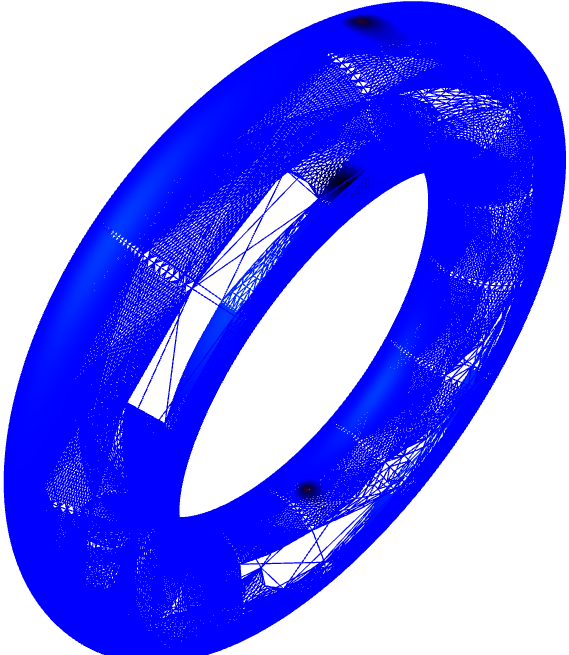
\includegraphics[width=0.5\textwidth]{criticos_toro}
		\caption{Puntos críticos de la función altura en el toro (zonas oscuras).}
	\end{minipage}
 		\label{fig:morse_toro}
\end{figure}	

Se pueden ver los puntos críticos en color negro, aunque sólo se pueden observar $3$ de los $4$ existentes para el toro ya que al ser una superficie opaca sólo se pueden ver los ocultos en modo malla y dependiendo de la posición de la cámara (se ha intentado capturar la escena en la que aparezcan el mayor nº de puntos críticos posible).

\section*{Vías futuras}

\subsection*{Resultados importantes}
Los hechos definidos por Allen Hatcher en su artículo son de gran interés y pueden aportar mucha información para el suavizado de estructuras topológicas. Aunque es cierto que tales resultados están orientados específicamente para la demostración de los $2$ resultados, se podrían utilizar para simplificar otras demostraciones del campo de la topología diferencial, siempre que traten variedades topológicas $2$-dimensionales.\\

\subsection*{Teselación Phong}
Para complementar el modelo de iluminación Phong, sería interesante probar a añadir $1$ o $2$ niveles de teselado en el que se implemente la teselación Phong \cite{PhongTess}. Los nuevos vértices generados en dichos niveles muy probablemente no estarán en la superficie, es decir, perdemos una característica bastante importante de la malla de triángulos generada.\\
\\Sin embargo, es la idónea para la iluminación Phong, por lo que si sólo se añaden unos pocos vértices los resultados visuales podrían mejorar, porque desparecerían en algunos casos las ``zonas de transición de luz'' (donde se aprecian colores planos aunque la transición entre ellos sea continua).\\
\\Se podría implementar en el Geometry shader, puesto que al ser una etapa posterior al Tessellation shader sería como añadir uno o varios niveles más de teselación. Es posible que la ganancia en calidad no fuese suficiente en comparación con la pérdida de eficiencia, pero para ello sería necesario estudiarlo a fondo.\\

\subsection*{Transform feedback}
El estudio de la teselación podría continuar por la técnica de ``Transform feedback'', que permite procesar de nuevo la malla generada como salida tras el teselado. Se podría implementar un teselado incremental, de manera similar a una función recursiva, es decir, subdividir triángulos hasta que se llegue al punto deseado (GLSL no permite recurrencias de forma natural). Intuitivamente parece que consumirá bastantes recursos, pero puede que gestione mejor los recursos disponibles, incluso se podrían eliminar etapas de la secuencia de renderizado (los Tessellation shaders no harían falta, bastaría con el Geometry shader, aunque habría que estudiar la eficiencia).\\

\subsection*{Funciones de Morse}
Una funcionalidad que se podría añadir al programa en un futuro, es la visualización de una función de Morse para una superficie dada. Aprovechando que podemos definir una superficie mediante cartas, podemos mostrar datos interesantes de cualquier función de Morse que tenga como dominio dicha superficie, tales como puntos críticos e ``isobaras''. Los puntos críticos son fácilmente calculables teniendo en cuenta que si para una carta $\phi$ y una función de Morse $f$, tomando $g(u,v)=f \circ \phi (u,v)$, si tiene derivadas parciales iguales a $0$ en $p=\phi(u,v)$ y $p$ es un valor regular de $\phi$, entonces $p$ es un punto crítico de $f$.\\
\\Teniendo en cuenta el lema $2.1$ del apartado de Teoría de Morse (parte I), se puede decir que nuestro programa actualmente es capaz de visualizar cualquier función de Morse si a las cartas a representar se les aplica previamente un embebimiento adecuado en $\R^3$ (ya que la función de Morse coincidiría con la función altura), aunque la superficie también se visualizaría a través de dicho embebimiento (puede aplicar una deformación drástica a la superficie). Es decir, la teoría apoya la posibilidad de representar cualquier función de Morse con domino una superficie de $\R^3$, pero visualmente sería incomprensible.\\
\\Para mejorar la visualización de los puntos críticos se podría añadir la funcionalidad de teselar sólo cerca de los puntos críticos, cuando se estén visualizando, para que se detecten con mayor precisión. Adicionalmente se podría renderizar la superficie controlando su opacidad, para así poder ver todos los puntos críticos a la vez, aunque estén en caras ocultas.

\subsection*{WebGL}
En cuanto a la portabilidad se podría estudiar implementarlo para sistemas operativos Windows o incluso hacer una versión web con WebGL.\\

\subsection*{Superficies estáticas}
A priori, el programa implementado sólo sirve para visualizar con cierto nivel de precisión una superficie u homotopía, pero haciendo un correcto uso de la secuencia de renderizado se podría aprovechar para generar objetos $3D$ estáticos, es decir, dada una parametrización de entrada, obtener como salida una malla indexada en la que los triángulos están concentrados en aquellas zonas más complejas de la superficie. De esta forma podríamos cargar en un futuro dicha superficie sin tener que evaluar en cada frame la parametrización.\\
\\Para completar lo anterior se podría estudiar el generar junto a dicha malla indexada un mapa de normales, de esta manera la superficie se visualizaría mucho mejor en cuanto a iluminación sin empeorar drásticamente el rendimiento. Esta funcionalidad sería idónea para generar mallas indexadas que aproximen a una cierta superficie y que se utilizarán en una escena $3D$. También se podría completar con otras técnicas de teselado para aumentar el rendimiento cuando haya varios objetos en la escena y estén a distintas (visualizar el objeto real cuando esté cerca y la malla inicial cuando supere una cierta distancia).\\
\\En este caso si sería interesante estudiar a fondo el post-procesado de vértices, sobretodo para reducir los triángulos utilizados en zonas similares al plano. Por ejemplo, si queremos mostrar una función que perturba el plano en zonas aisladas, como la parametrización de ejemplo ``waves$2$.in'', se utilizarían muy pocos triángulos en las zonas totalmente planas y el resto se usarían en las zonas complementarias, independientemente del tamaño de la malla inicial (actualmente las zonas planas están trianguladas según la malla inicial).

\endinput
